\documentclass[12pt]{beamer}
\usetheme{Madrid}
\usepackage[utf8]{inputenc}
\usepackage[french]{babel}
\usepackage[T1]{fontenc}
\usepackage{amsmath}
\usepackage{amsfonts}
\usepackage{amssymb}
\usepackage{graphicx}
\usepackage{listings}
\usepackage{xcolor}

\definecolor{codegreen}{rgb}{0,0.6,0}
\definecolor{codegray}{rgb}{0.5,0.5,0.5}
\definecolor{codepurple}{rgb}{0.58,0,0.82}
\definecolor{backcolour}{rgb}{0.95,0.95,0.92}

\lstdefinestyle{mystyle}{
    backgroundcolor=\color{backcolour},   
    commentstyle=\color{codegreen},
    keywordstyle=\color{magenta},
    numberstyle=\tiny\color{codegray},
    stringstyle=\color{codepurple},
    basicstyle=\ttfamily\footnotesize,
    breakatwhitespace=false,         
    breaklines=true,                 
    captionpos=b,                    
    keepspaces=true,                 
    numbers=left,                    
    numbersep=5pt,                  
    showspaces=false,                
    showstringspaces=false,
    showtabs=false,                  
    tabsize=2
}
\lstset{style=mystyle}

\usepackage{multido}
\newcommand{\myrepeat}[2]{%
    \newcount\iterations%
    \iterations #1%
    \advance\iterations -1
    \multido{\iN=0+1}{\iterations}{#2\ }#2%
}
\setcounter{tocdepth}{4}
\setcounter{secnumdepth}{4}
\author{TRAN-THUONG Tien-Thinh}
\title{Algorithme de Knuth-Morris-Pratt KMP}
%\setbeamercovered{transparent} 
%\setbeamertemplate{navigation symbols}{} 
%\logo{} 
%\institute{} 
%\date{} 
%\subject{} 
\begin{document}

\begin{frame}
\titlepage
\end{frame}

\begin{frame}{Présentation}
\tableofcontents
\end{frame}

\section{Utilité}
\begin{frame}{Utilité}
\begin{block}{1977}
Publication de l'article en 1977 : \\
• Donald Knutt (The Art of Computer Programming) \\
• James Morris \\
• Vaughan Pratt \\
\end{block}
\begin{block}{L'algorithme KMP}
Un algorithme de recherche d'une chaîne de caractères $P$ (Pattern) de taille $p$ au sein d'une autre chaîne $S$ (String) de taille $s$ avec $p \leq s$. \\
• L'algorithme Naïf est en $O(s \times p) $ \\
• KMP est en $O(s) $
\end{block}
\end{frame}

\section{Algorithme Naïf}
\begin{frame}{Algorithme Naïf}
\lstinputlisting[language=Python, firstline=4, lastline=19]{../main.py}
Le pire cas est en $O\ (s \times p)$
\end{frame}

\section{KMP}
\subsection{Exemple simple}
\begin{frame}{KMP - Exemple}
\begin{tabular}{ l || p{0.01cm}p{0.01cm}p{0.01cm}p{0.01cm}p{0.01cm}p{0.01cm}p{0.01cm}p{0.01cm}p{0.01cm}p{0.01cm}p{0.01cm}p{0.01cm}p{0.01cm}p{0.01cm}p{0.01cm}p{0.01cm}p{0.01cm}p{0.01cm}p{0.01cm}p{0.01cm}p{0.01cm}p{0.01cm}p{0.01cm}} 
   S  &A&B&C& &A&B&C&D&A&B& &A&B&C&D&A&B&C&D&A&B&D&E \\ \hline
   P  &A&B&C&D&A&B&D  \\ 
      &O&O&O&X \\ \hline
   P  & & & & &A&B&C&D&A&B&D \\
   	  & & & & &O&O&O&O&O&O&X \\
   >  & & & & & & & & &A&B&C&D&A&B&D \\
   	  & & & & & & & & &O&O&X \\ \hline
   P  & & & & & & & & & & & & & & & &A&B&C&D&A&B&D \\
      & & & & & & & & & & & & & & & &O&O&O&O&O&O&O  
\end{tabular} \\
L'idée est de mettre en place un tableau pour Pattern permettant de ne pas devoir traiter plusieurs fois un même caractère.
\end{frame}


\subsection{Tableau}
\begin{frame}{KMP - Tableau}
\begin{center}
\begin{tabular}{ l || p{0.01cm}p{0.01cm}p{0.01cm}p{0.01cm}p{0.01cm}p{0.01cm}p{0.01cm}p{0.01cm}p{0.01cm}p{0.01cm}p{0.01cm}p{0.01cm}p{0.01cm}p{0.01cm}p{0.01cm}p{0.01cm}p{0.01cm}p{0.01cm}p{0.01cm}p{0.01cm}p{0.01cm}p{0.01cm}p{0.01cm}p{0.01cm}} 
   Indice  &0&1&2&3&4&5&6 \\
   Pattern P &A&B&C&D&A&B&D  \\ \hline
   Tableau T &0&0&0&0&1&2&0
\end{tabular}
\end{center}
\lstinputlisting[language=Python, firstline=24, lastline=35]{../main.py}
\end{frame}

\begin{frame}{KMP - Tableau exemple}
\begin{center}
\begin{tabular}{ l || p{0.01cm}p{0.01cm}p{0.01cm}p{0.01cm}p{0.01cm}p{0.01cm}p{0.01cm}p{0.01cm}p{0.01cm}p{0.01cm}p{0.01cm}p{0.01cm}p{0.01cm}p{0.01cm}p{0.01cm}p{0.01cm}p{0.01cm}p{0.01cm}p{0.01cm}p{0.01cm}p{0.01cm}p{0.01cm}p{0.01cm}p{0.01cm}} 
   Pattern P &A&B&C&D&A&B&D  \\
   Tableau T &0&0&0&0&1&2&0
\end{tabular}
\end{center}
\lstinputlisting[language=Python, firstline=37, lastline=38]{../main.py}

\begin{center}
\begin{tabular}{ l || p{0.01cm}p{0.01cm}p{0.01cm}p{0.01cm}} 
   Pattern P &A&A&A&B  \\
   Tableau T &0&1&2&0
\end{tabular}
\end{center}
\lstinputlisting[language=Python, firstline=39, lastline=40]{../main.py}

\begin{center}
\begin{tabular}{ l || p{0.01cm}p{0.01cm}p{0.01cm}p{0.01cm}p{0.01cm}p{0.01cm}p{0.01cm}p{0.01cm}p{0.01cm}p{0.01cm}p{0.01cm}p{0.01cm}p{0.01cm}p{0.01cm}p{0.01cm}p{0.01cm}p{0.01cm}p{0.01cm}p{0.01cm}p{0.01cm}p{0.01cm}p{0.01cm}p{0.01cm}p{0.01cm}} 
   Pattern P &A&B&B&A&B  \\
   Tableau T &0&0&0&1&2
\end{tabular}
\end{center}
\lstinputlisting[language=Python, firstline=41, lastline=42]{../main.py}
\end{frame}

\subsection{Recherche}
\begin{frame}{KMP - Recherche}
\lstinputlisting[language=Python, firstline=48, lastline=65]{../main.py}
\end{frame}
\begin{frame}{KMP - Exemple de recherche}
\lstinputlisting[language=Python, firstline=67, lastline=74]{../main.py}
\end{frame}

\subsection{Automate}
\begin{frame}{KMP - Automate}
\begin{center}

S : ABC ABCDAB ABCDABCDABDE \\
\end{center}

\begin{center}
\begin{tabular}{ l || p{0.01cm}p{0.01cm}p{0.01cm}p{0.01cm}p{0.01cm}p{0.01cm}p{0.01cm}p{0.01cm}p{0.01cm}p{0.01cm}p{0.01cm}p{0.01cm}p{0.01cm}p{0.01cm}p{0.01cm}p{0.01cm}p{0.01cm}p{0.01cm}p{0.01cm}p{0.01cm}p{0.01cm}p{0.01cm}p{0.01cm}p{0.01cm}} 
   Pattern P &A&B&C&D&A&B&D \\
   Tableau T &0&0&0&0&1&2&0 \\
\end{tabular}
\end{center}
\begin{figure}
	\centering
    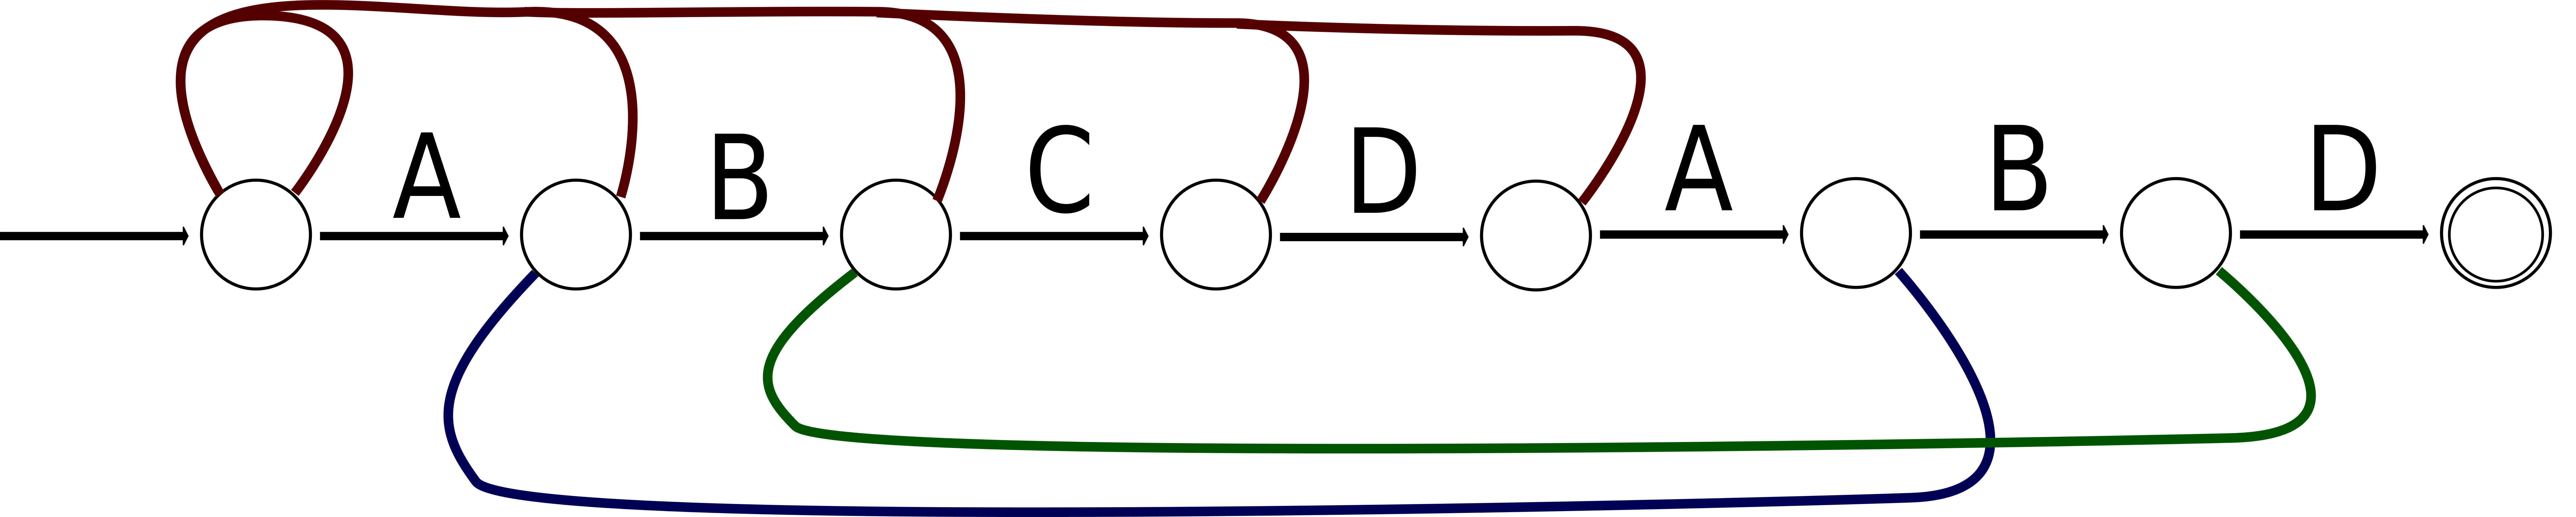
\includegraphics[width=320px]{Schema/Automate.png}
	\caption{Schéma automate}
\end{figure}
\end{frame}

\end{document}
